\documentclass[10pt]{standalone}
\usepackage{amsmath}
\usepackage{amssymb}
\usepackage[utf8]{inputenc}
\usepackage{pgf,tikz,pgfplots}
\pgfplotsset{compat=1.15}
\usetikzlibrary{arrows}
\pagestyle{empty}
\begin{document}

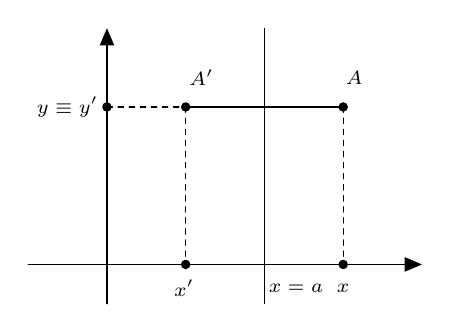
\begin{tikzpicture}[line cap=round,line join=round,>=triangle 45,x=1.0cm,y=1.0cm]
\draw[->] (-1.,0.) -- (4.,0.);
;
\draw[->] (0.,-0.5) -- (0.,3.);

\clip(-1.,-0.5) rectangle (4.,3.);
\draw  (2.,-1.) -- (2.,3.);
\draw  (1.,2.)-- (3.,2.);
\draw [dash pattern=on 2pt off 2pt] (0.,2.)-- (1.,2.);
\draw [dash pattern=on 2pt off 2pt] (1.,2.)-- (1.,0.);
\draw [dash pattern=on 2pt off 2pt] (3.,2.)-- (3.,0.);
\begin{scriptsize}
%\draw[color=black] (1.74,6.17) node {$f$};
\draw [fill=black] (3.,2.) circle (1.5pt);
\draw[color=black] (3.14,2.37) node {$A$};
\draw [fill=black] (1.,2.) circle (1.5pt);
\draw[color=black] (1.2,2.37) node {$A'$};

\draw [fill=black] (0.,2.) circle (1.5pt);
\draw[color=black] (-0.5,2.0) node {$y\equiv y'$};
\draw [fill=black] (1.,0.) circle (1.5pt);
\draw[color=black] (0.98,-0.3) node {$x'$};
\draw [fill=black] (3.,0.) circle (1.5pt);
\draw[color=black] (3.,-0.3) node {$x$};
\draw[color=black] (2.4,-0.3) node {$x=a$};

\end{scriptsize}
%\end{axis}
\end{tikzpicture}
\end{document}